% VLDB template version of 2020-08-03 enhances the ACM template, version 1.7.0:
% https://www.acm.org/publications/proceedings-template
% The ACM Latex guide provides further information about the ACM template

\documentclass[sigconf, nonacm]{acmart}

\usepackage{amsmath}
\newtheorem{definition}{Definition}
\usepackage{bbding}
\usepackage{booktabs}
\usepackage{graphicx}
\usepackage{subcaption}
\usepackage{balance}
\usepackage{hyperref}
\usepackage{minted}
\usepackage[inline]{enumitem}
\usepackage{tikz}
\usetikzlibrary{arrows.meta}
\usepackage[linesnumbered,ruled,noend]{algorithm2e}
\SetKwInOut{Input}{input}\SetKwInOut{Output}{output}
\SetKwProg{Fn}{function}{}{end}
\SetKwSwitch{Match}{Case}{Other}{match}{do}{case}{otherwise}{endcase}

%% The following content must be adapted for the final version
% paper-specific
\newcommand\vldbdoi{XX.XX/XXX.XX}
\newcommand\vldbpages{XXX-XXX}
% issue-specific
\newcommand\vldbvolume{14}
\newcommand\vldbissue{1}
\newcommand\vldbyear{2021}
% should be fine as it is
\newcommand\vldbauthors{\authors}
\newcommand\vldbtitle{\shorttitle}
% leave empty if no availability url should be set
\newcommand\vldbavailabilityurl{http://vldb.org/pvldb/format_vol14.html}
% whether page numbers should be shown or not, use 'plain' for review versions, 'empty' for camera ready
\newcommand\vldbpagestyle{plain}

\begin{document}
\title{Out-of-Core Property Graph Matching for Real-World Graph Databases}

%%
%% The "author" command and its associated commands are used to define the authors and their affiliations.
\author{Yanxuan Cui}
\affiliation{%
  \institution{Tsinghua University}
  \city{Being}
  \state{China}
  \postcode{100084}
}
\email{cuiyx18@mails.tsinghua.edu.cn}

\begin{abstract}
  Property graph matching is the most important operation of graph database and has a wide range of applications.
  The problem has been studied extensively, however, on oversimplified graph models.
  Because of the complexity involving directions, multi-edges, labels in property graphs,
  optimizations aimed at simple graphs are not suitable to handle the storage and matching problem of property graphs.
  Moreover, existing approaches rely on huge memory resources to run their system and hinder the popularity of graph technology.

  We present SeqStar, the first out-of-core property graph matching system that can execute real-world complex queries efficiently.
  The storage engine of SeqStar uses a novel \emph{vertex-centric} storage model.
  By storing necessary information together with the vertices,
  SeqStar avoids the random disk access problem of existing work.
  In the graph matching engine, we propose a novel star decomposition algorithm that preserves all the relevant filtering information on stars.
  Therefore, SeqStar can filter out more unnecessary matchings in the very beginning.
  To reduce the memory usage, SeqStar compresses the intermediate results from star matching and performs pipeline join on the compressed data.
  Moreover, we propose a predicate pushdown method for SeqStar to optimize real-world queries.
\end{abstract}


\maketitle

%%% do not modify the following VLDB block %%
%%% VLDB block start %%%
\pagestyle{\vldbpagestyle}
\begingroup\small\noindent\raggedright\textbf{PVLDB Reference Format:}\\
\vldbauthors. \vldbtitle. PVLDB, \vldbvolume(\vldbissue): \vldbpages, \vldbyear.\\
\href{https://doi.org/\vldbdoi}{doi:\vldbdoi}
\endgroup
\begingroup
\renewcommand\thefootnote{}\footnote{\noindent
This work is licensed under the Creative Commons BY-NC-ND 4.0 International License. Visit \url{https://creativecommons.org/licenses/by-nc-nd/4.0/} to view a copy of this license. For any use beyond those covered by this license, obtain permission by emailing \href{mailto:info@vldb.org}{info@vldb.org}. Copyright is held by the owner/author\@(s). Publication rights licensed to the VLDB Endowment. \\
\raggedright{} Proceedings of the VLDB Endowment, Vol. \vldbvolume, No. \vldbissue\ %
ISSN 2150--8097. \\
\href{https://doi.org/\vldbdoi}{doi:\vldbdoi} \\
}\addtocounter{footnote}{-1}\endgroup
%%% VLDB block end %%%

%%% do not modify the following VLDB block %%
%%% VLDB block start %%%
\ifdefempty{\vldbavailabilityurl}{}{
\vspace{.3cm}
\begingroup\small\noindent\raggedright\textbf{PVLDB Artifact Availability:}\\
The source code, data, and/or other artifacts have been made available at \url{\vldbavailabilityurl}.
\endgroup
}
%%% VLDB block end %%%
\section{Introduction}
Graph matching
%~\footnote{There are two kinds of graphs in a graph matching problem: one is the large \emph{data graph}, the other is the much smaller \emph{pattern graph}}
is one of the most important applications of graph databases. In graph matching, a relative small \emph{pattern graph} is used to match subgraphs of a relative large \emph{data graph}.
It is widely used in many fields,
such as Twitter's recommendation systems~\cite{DBLP:journals/pvldb/GuptaSGGZLL14,DBLP:journals/pvldb/SharmaJBLL16},
electronic computer-aided design~\cite{DBLP:conf/dac/OhlrichEGS93},
and protein-protein interaction (PPI) networks~\cite{milenkovic2008uncovering}.
Nowadays, users of industrial graph databases such as Neo4j\footnote{\url{https://neo4j.com}}
can easily model data as property graphs and expressing their queries via the Cypher~\cite{DBLP:conf/sigmod/FrancisGGLLMPRS18} query language.
Although it is convenient to use, the matching process of these industrial graph databases are time and resource consuming.
Many novel subgraph matching algorithms have been proposed~\cite{DBLP:journals/pvldb/SunWWSL12,DBLP:conf/sigmod/HanLL13,DBLP:conf/sigmod/ShaoCCMYX14,DBLP:conf/cloud/SerafiniMS17,DBLP:journals/pvldb/QiaoZC17,DBLP:conf/sigmod/DiasTGM019}, with even orders of magnitude of speedup compared to the industrial graph databases.
However, there are two gaps that hinder these algorithms from being widely adopted in the real-world scenarios:
(1) the gap between the complexity of real-world queries and the simplicity of graphs that the existing algorithms can handle;
(2) the huge memory and high-speed network requirements for the existing algorithms to query on large graphs and the limitation of resource budget.

The property graph is the de facto graph model for real-world graph matching problems.
A property graph is a directed graph with labels attached to vertices and edges.
There may be multiple edges connecting two vertices and even edges for self-loop (edges connecting back to their source vertices).
Moreover, users usually provide extra searching conditions via the WHERE clause~\cite{DBLP:journals/csur/AnglesABHRV17}. However,  current studies mostly deal with simple graph models such as ignoring the directions, labels, or multi-edges. WHERE clause is not considered either~\cite{DBLP:journals/pvldb/SunWWSL12,DBLP:conf/sigmod/HanLL13,DBLP:conf/sigmod/KimLBHLKJ16,DBLP:journals/pvldb/QiaoZC17,DBLP:journals/pvldb/MhedhbiS19}. The optimizations aimed at simple graphs usually heavily rely on the equivalence of vertices~\cite{DBLP:conf/sigmod/HanLL13,DBLP:journals/pvldb/QiaoZC17}, which is harder to find in a property graph because of the complexity of directions and labels. Moreover, in the implementation level, the storage engine designed for simple graph models encounters excessive random disk seeks when matching a real-world property graph.

%This limitation is not only a matter of engineering,
%but also a serious algorithm problem:
%(1) the storage engine designed for simple graph may encounter superfluous random disk reads when matching a property graph;
%(2) the optimizations aimed at simple graph usually rely heavily on the equivalence of vertices~\cite{DBLP:conf/sigmod/HanLL13,DBLP:journals/pvldb/QiaoZC17}, which is harder to find in a property graph because of the complexity of directions and labels.

Existing algorithms rely on main memory for their computation. It is extremely uneconomic for property graph matching problem. The memory needs to hold not only the graph data but also the intermediate results which grow exponentially with respect to the size of graph data. Our experiment shows that a graph with $6.9 \times 10^{7}$ edges could generate $1.7 \times 10^{13}$ rows of matching results.
%(1) The memory needs to hold not only the data graph, but also the intermediate result which grows exponentially with respect to the size of the data graph, as our experiment shows that a graph with $6.9 \times 10^{7}$ edges could generate $1.7 \times 10^{13}$ rows of matching results.
Existing systems~\cite{DBLP:conf/sosp/TeixeiraFSSZA15,DBLP:conf/sigmod/DiasTGM019,DBLP:journals/pvldb/MhedhbiS19} require hundreds of GB of memory to process such graphs. Therefore, we resort to use external memory (such as SSDs) to support property graph matching.
%(2) For distributed approaches, on the one hand it is hard to partition the graph across cluster machines to minimize the communication cost~\cite{DBLP:journals/im/LeskovecLDM09} and have performance problems~\cite{DBLP:conf/sigmod/KimLBHLKJ16},
%one the other hand it is inconvenient and costly for the end user to maintain the cluster nodes~\cite{DBLP:conf/osdi/KyrolaBG12}.

This paper proposes SeqStar, a high performance out-of-core property graph matching system for real-world graphs, which scans the disk sequentially by matching stars (a star contains a root vertex and some leaves which are the neighbors of the root).

%Therefore, in order to match up with the need of real-world problems,a high performance disk-based property graph matching system is desirable.

\subsection*{Contributions}
There are two fundamental components in SeqStar:
the graph storage engine and the graph matching engine. Both are designed specificly to deal with the graph machine problem efficiently.

The storage engine in SeqStar uses the \emph{vertex-centric storage model} which stores the information related to a specific vertex together.
The conventional way to store graphs is the compressed sparse row (CSR) and compressed sparse column (CSC) approach which stores in/out-edges \emph{separately}~\cite{DBLP:conf/sc/PearceGA10,DBLP:conf/osdi/KyrolaBG12}.
CSR is equivalent to storing the graph as adjacency list: the out-edges are stored consecutively on disk.
And CSC stores the in-edges in a similar manner.
In contrast, SeqStar stores the graph data by storing the in/out-edges \emph{together} with the neighbors of each vertex.
With small indexes on disks, pattern matching can quickly get the correct address of relevant data on disk during pattern matching.
We also provide two convenient iterator interfaces to interact with the storage engine.
As a result, SeqStar can avoid random disk seeks and perform graph matching in a sequential disk scan.

For the graph matching engine, SeqStar uses a star decomposition based algorithm to run graph matching.
The analyzer of SeqStar analyzes the graph matching query and select a vertex-cover heuristically as the roots of stars.
%这里加一句如何把原图分解为星型子图
We save all useful filtering information in each star subgraph after decomposition. To reduce the amount of memory that would be used as the storage of intermediate results, a novel compression method, which postponing Cartesian production and digging equivalence classes, is used for star matching results. SeqStar's efficient and scalable pipeline join algorithm is able to process the compressed data. To the best of our knowledge, SeqStar is the first system that integrates the optimization of WHERE clauses in the graph matching algorithm, by pushing the predicates down to the star matching process.

According to our experiments, SeqStar outperforms the state-of-the-art graph querying system Graphflow by up to $26\times$.
And SeqStar can run the queries that Graphflow fails to run due to the out of memory problem.
For complex property graphs that existing academic researches do not support,
we compare SeqStar with industrial graph database Neo4j, and achieved over $2100\times$ speedup.
%To reduce memory usage, we make the following contributions:
%(1) a novel star decomposition algorithm that keeps all the useful filtering information in stars,
%(2) a novel compression algorithm for stars' matching results by postponing Cartesian production and digging equivalence classes,
%(3) an efficient and scalable pipeline join algorithm that is able to process the compressed data directly.

%Moreover, to the best of our knowledge, we are the first one to integrate the optimization of WHERE clauses in the graph matching algorithm, by pushing the predicates down to the star matching process.
%% The conventional graph storage method is the compressed sparse column (CSC) and the compressed sparse row (CSR) format~\cite{DBLP:conf/osdi/KyrolaBG12},
%% which stores the in/out-edges separately for each vertex.
%% However, because of the multi-edges in property graphs, the in/out-edges have to be searched many times to check the matching of a vertex, and result in excessive random disk seeks.
%% To address this challenge, we propose the \emph{vertex-centric storage model} that stores all the necessary information together with the vertices, such that the vertices could be matched in a single sequential scan.

%% Generally speaking, there are two kinds of graph isomorphism algorithm,
%% differing on whether intermediate results are materialized.
%% The first is the backtracking tree-searching method~\cite{DBLP:journals/jacm/Ullmann76,DBLP:journals/pvldb/LeeHKL12,DBLP:conf/sigmod/HanLL13,DBLP:conf/sigmod/KimLBHLKJ16},
%% which does not generate intermediate results but have scaling problems~\cite{DBLP:conf/cloud/SerafiniMS17}.
%% The second is the join-based algorithm~\cite{DBLP:journals/pvldb/LaiQLC15,DBLP:journals/pvldb/QiaoZC17,DBLP:journals/pvldb/SunWWSL12,DBLP:journals/pvldb/MhedhbiS19},
%% which decomposes the pattern graph into smaller matching unit and materialize the intermediate results,
%% and the final result is obtained by joining on these intermediate results.
%% Because of the notorious poor locality of graphs,
%% enormous amount of random disk accesses would be encountered for an out-of-core tree-searching approach.
%% Based on this observation, this paper designs a join-based property graph matching algorithm.

%% The most fundamental problem of a graph matching algorithm is to determine the basic matching unit.
%% Edges are the simplest matching units, however, intermediate results much larger than the data graph would be generated and result in costly join operations.
%% To avoid excessive joins, authors use more complex structures i.e.,
%% frequent subgraphs, multi-hop edges, or cliques as their matching unit~\cite{DBLP:conf/sigmod/HeS08,DBLP:conf/edbt/ZhangLY09,DBLP:journals/pvldb/QiaoZC17}, however,
%% these algorithms rely on super-linear indices~\cite{DBLP:journals/pvldb/SunWWSL12}.
%% To address this challenge, we make a balance by choosing stars as our basic unit.
%% And our star decomposition algorithm is enhanced such that the stars keep as much filtering information as possible.
%% Our experiment shows that this enhancement could reduce the intermediate results by up to $43\%$ of the existing works.

%% However, the stars' matching results could still be very large because the matching results grow exponentially with respect to the data graph,
%% e.g., a 129M graph could easily eat up hundreds or even thousands GB of memory to store the intermediate results.
%% Inspired by VCBC~\cite{DBLP:journals/pvldb/QiaoZC17}, we develop a novel compression algorithm for star' matching result by postponing the costly Cartesian product and digging the equivalence classes in the leaves of the star.
%% The compression ratio is quite impressive, as high as $10^8$,
%% and we find that the size of the compressed star's matching results takes less than $23\%$ the space to store the graph,
%% which can even fit into the main memory of a laptop.

\section{Background}\label{sec:background}
This section introduces the formal definition of property graphs, and then discusses the property graph matching problem.
\subsection{Property Graph Model}
A \emph{property graph} is a directed vertex-labeled edge-labeled multigraph with self-edges,
and key-value properties are stored on vertices and edges.
We now provide the formal definition of a property graph.
\begin{definition}[Property Graph~\cite{DBLP:journals/csur/AnglesABHRV17}]
  A property graph $G$ is a tuple $(V, E, \rho, \lambda, \sigma)$, where:
  \begin{enumerate}[noitemsep,label={(\arabic*)}]
  \item $V$ is a finite set of vertices.
  \item $E$ is a finite set of edges such that $V$ and $E$ have no elements in common.
  \item $\rho: E \rightarrow (V \times V)$ is a total function.
    Intuitively, $\rho(e) = (v_1, v_2)$ indicates that $e$ is a directed edge from $v_1$ to $v_2$.
  \item $\lambda :(V \cup E) \rightarrow L$ is a total function where $L$ is a set of labels.
    Intuitively, if $v \in V, \rho(v) = l$ (respectively, $e \in E, \rho(e) = l$),
    then $l$ is the label of vertex $v$ (respectively, edge $e$).
  \item $\sigma: (V \cup E) \times Prop \rightarrow Val$ is a partial function with $Prop$ a finite set of properties and $Val$ a set of values.
    Intuitively, if $v \in V, p \in Prop, \sigma(v, p) = s$ (respectively, $e \in E, p \in Prop, \sigma(e, p) = s$),
    then $s$ is the value of property $p$ for vertex $v$ (respectively, edge $e$) in the property graph $G$.
  \end{enumerate}
\end{definition}
For simplicity, in this paper, we do not discuss the properties i.e., $\sigma$ in $G$,
because similar techniques can be used as processing the labels $\lambda$.
Thus, the property graph $G$ can be denoted by $(V(G), E(G), \rho_G, \lambda_G)$.
Please note that the total function $\rho_G$ is necessary, in general,
we cannot identify an edge simply by the starting and ending vertices such as $(u_1, u_2)$ as can be done in the simple graph model,
because multiple edges may appear between the two vertices.
However, we may use the $(u_1, u_2)$ notation if all we care about is that there exist at least one edge between $u_1$ and $u_2$.
\begin{definition}[Vertex Cover]
  A vertex cover $V_c$ of a property graph $G$ is a subset of $V(G)$ such that
  $\forall e \in E(G), \rho_G(e) = (u, v) \implies u \in V_C \lor v \in V_C$.
\end{definition}
\subsection{Property Graph Matching Problem}
\begin{definition}[Subgraph]
  A property graph $F$ is called a subgraph of a property graph $G$, written $F \subseteq G$, if
  $V(F) \subseteq V(G)$, $E(F) \subseteq E(G)$, $\rho_F$ is a restriction of $\rho_G$, and $\lambda_F$ is a restriction of $\lambda_G$.
\end{definition}
Let $G$ be any property graph, and let $S \subseteq V(G)$, then the \emph{induced subgraph} $G[S]$ is the graph whose vertex set is $S$ and whose edge set consists of all of the edges in $E(G)$ that have both endpoints in $S$.
\begin{definition}[Property Graph Isomorphism]
  Two property graphs $G$ and $H$ are isomorphic, written $G \cong H$,
  if there exists bijections $\theta: V(G) \rightarrow V(H)$ and $\phi: E(G) \rightarrow E(H)$ such that
  $\rho_G(e) = (u, v)$ if and only if $\rho_H(\phi(e)) = (\theta(u), \theta(v))$,
  $\lambda_G(v) = \lambda_H(\theta(v))$ for all $v \in V(G)$
  and $\lambda_G(e) = \lambda_H(\phi(e))$ for all $e \in E(G)$;
  Such a pair of mappings is called an isomorphism between $G$ and $H$.
\end{definition}
The bijection $\theta: V(G) \rightarrow V(H)$ is the key in the definition of property graph isomorphism,
because the bijection $\phi: E(G) \rightarrow E(H)$ is straightforward if $\theta$ is fixed.
However, due to automorphism, where an \emph{automorphism} of a graph is an isomorphism of the graph to itself,
the bijection $\theta$ may not be unique.
\begin{definition}[Property Graph Matching]\label{def:property_graph_matching}
  Given a data property graph $D$, a pattern property graph $P$ and a searching condition $\psi: PG \rightarrow B$ with $PG$ the set of property graph and $B$ the set of Boolean values,
  the property graph matching problem is to report the set $\mathcal{I} = \{F | F \subseteq D, F \cong P, \psi(F) = true\}$.
\end{definition}
Authors of previous works usually omit the searching condition $\psi$ in their definition of graph matching~\cite{DBLP:conf/sigmod/ShaoCCMYX14,DBLP:journals/pvldb/LaiQLC15,DBLP:conf/sigmod/KimLBHLKJ16,DBLP:journals/pvldb/QiaoZC17}.
And they adopt a loosely related technique called \emph{symmetry-breaking}~\cite{DBLP:conf/recomb/GrochowK07},
which ensures there is a unique bijection $\theta: V(P) \rightarrow V(F)$ by providing a partial order on $V(P)$ after exploiting the automorphism of $P$.
However, as we have stated before, the WHERE clause is a ubiquitous part of the query language of a graph database.
Users of a real-world graph database usually provide their self-defined searching condition $\psi$ to filter out unnecessary matchings not only symmetry-breaking conditions.
Thus, the searching condition we defined here can be viewed as a super set of symmetry-breaking.
We add the searching condition in the definition because it is actually a part of the property graph matching problem,
and we also found that it can be decomposed and pushed down to lower phase to boost the evaluation of graph matching (Section~\ref{sec:framework}).

A property graph is always directed.
However, in some cases such as friendship, there is no need to pay attention to the directions of the edges.
In order to support this kind of relationship, a naive approach is to add a duplicate edge in opposite direction for each edge in the data graph.
More elegantly, we allow the pattern graph $P$ to contain undirected edges.
Users can simply ignore the direction by providing undirected edges in $P$ like in industrial graph databases such as Neo4j.

\section{Overview of SeqStar}\label{sec:framework}
We demonstrate the workflow of SeqStar in this section,
and use an example to show the query processing stages.
\subsection{SeqStar Workflow}
\begin{figure}[ht]
  \centering
  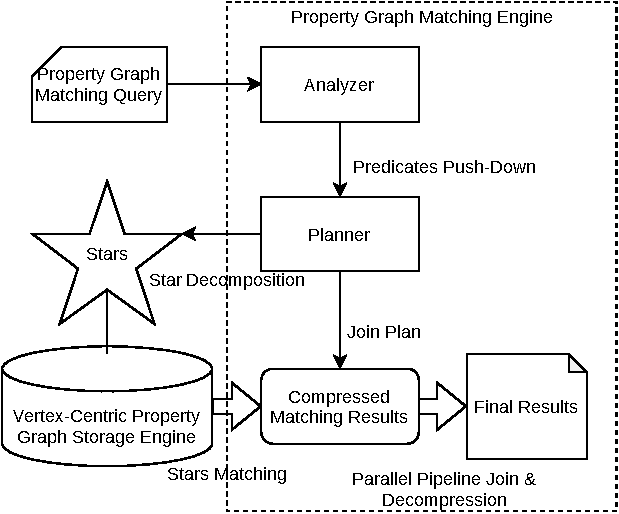
\includegraphics[width=0.48\textwidth]{img/architecture.pdf}
  \caption{SeqStar workflow.}\label{img:architecture}
\end{figure}
Figure~\ref{img:architecture} shows the workflow of SeqStar. There are mainly two building blocks in SeqStar: the storage engine and the property graph matching engine.
Both are specially designed to deal with the property graph matching problem efficiently.

Traditional graph storage engines such as used in graph databases store the in-edges and out-edges separately for each vertex.
Because of the complexity in property graphs,
such a storage method is not suitable and would incur many unnecessary random disk accesses.
We develop a vertex-centric property storage model to store all information related to one vertex together to address the problem (\S\ref{sec:storage}).


Based on the storage model,
we propose an efficient property graph matching engine that is able to execute real-world complex queries (\S\ref{sec:match}).
The core of the graph matching engine is the planner, which  decomposes the pattern into a series of stars.
Compared with existing works, we take a step further by introducing
(1) a matching result compression algorithm which reduces the cost of materializing intermediate results,
(2) a predicate pushdown optimizer that is able to filter out unnecessary matchings in early stages and mitigate the burden of the join process.
\subsection{Query Processing Stages}
Here is an example of how a concrete query gets executed in SeqStar.
Consider the Cypher (Neo4j's graph query language) query in Figure~\ref{img:cypher_query},
which generates the pattern graph in Figure~\ref{img:running_example} (b):

\begin{figure}[ht]
  \begin{Verbatim}[fontsize=\small]
    MATCH (u1:Person)-[:FOLLOWS]->(u2:Person)-[:FOLLOWS]->(u1),
          (u1)-[:FOLLOWS]->(u3:Person)-[:FOLLOWS]->(u1),
          (u1)-[:REPOSTS]->(u4:Media),
          (u2)-[:LIKES]->(u4)<-[:LIKES]-(u3)
    WHERE u2 > u1 AND NOT (u3 <= u1 OR u4 >= 8)
  \end{Verbatim}
  \caption{Example query.}\label{img:cypher_query}
\end{figure}

\begin{figure*}[ht]
  \centering
  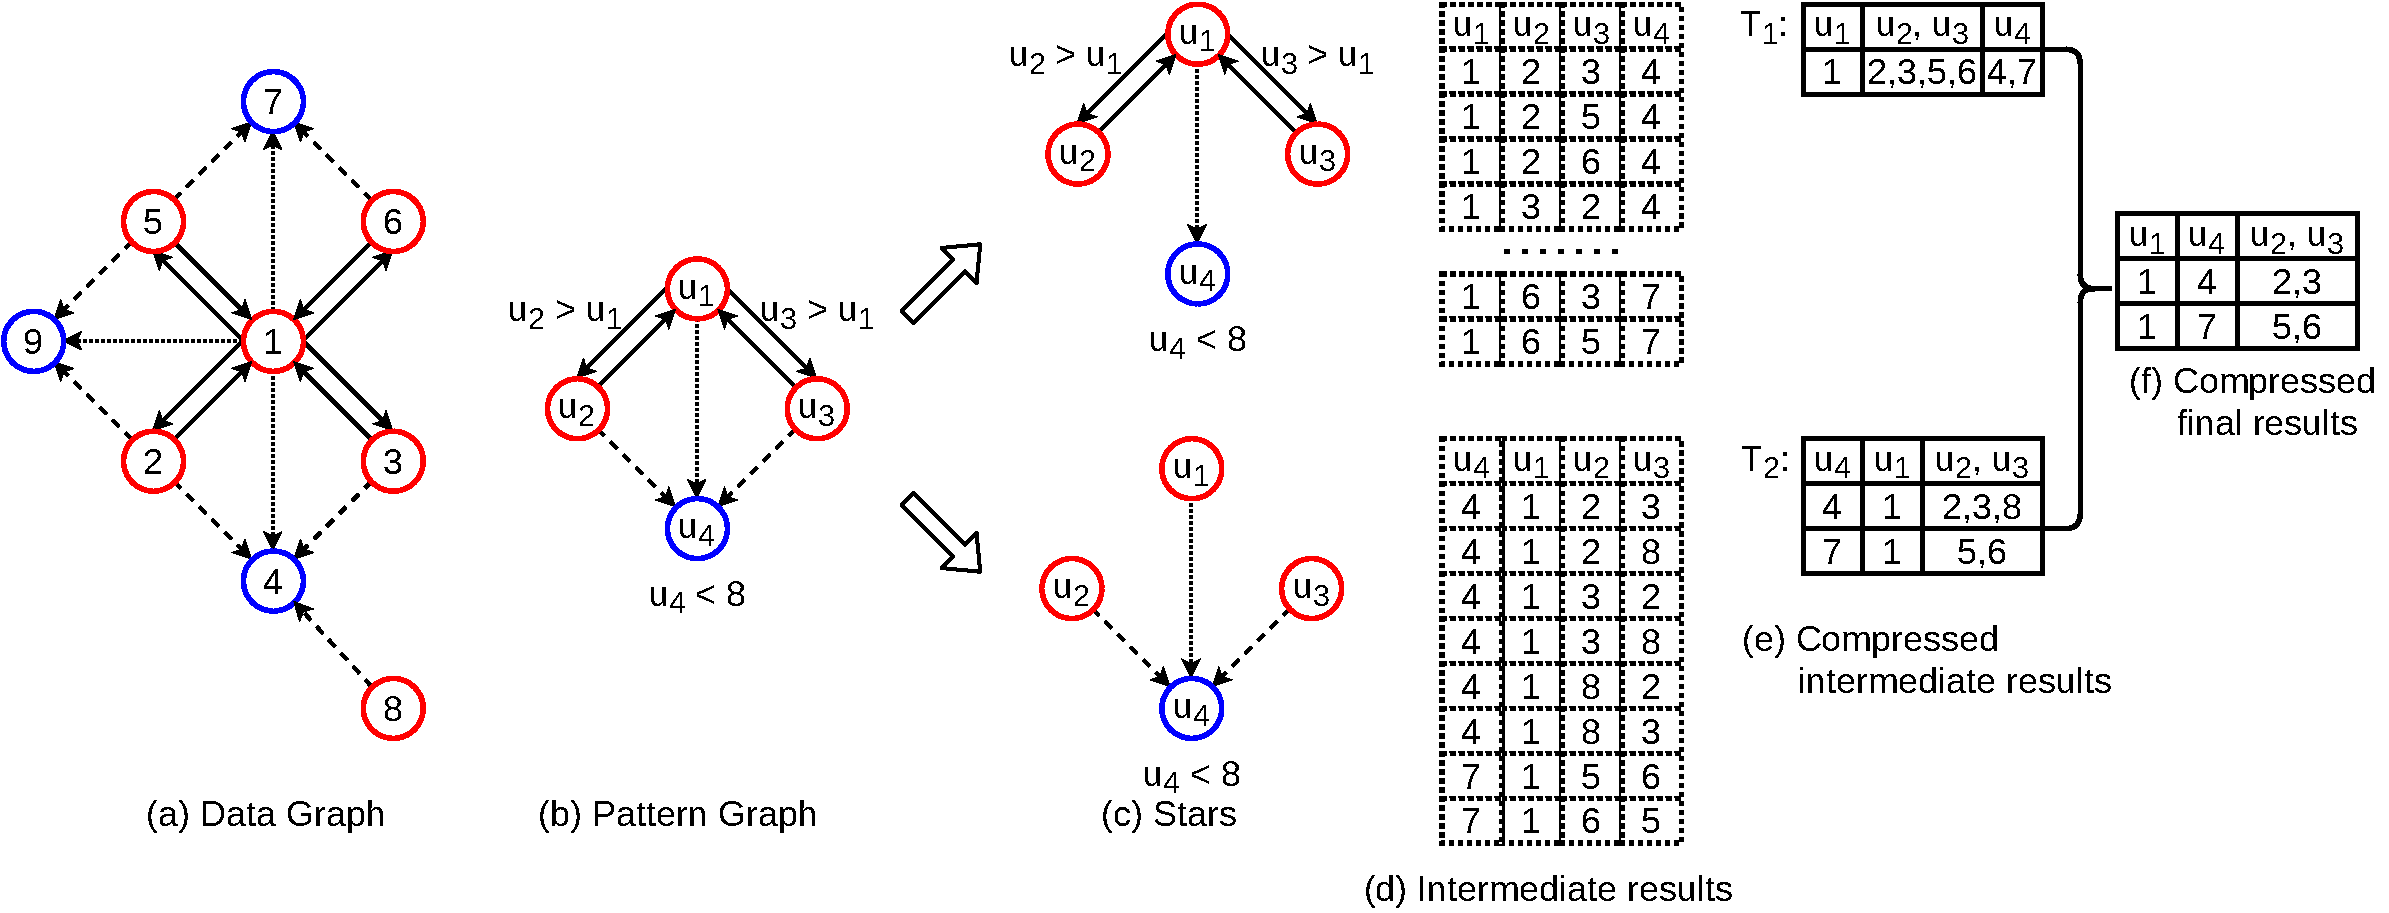
\includegraphics[width=\textwidth]{img/running_example.pdf}
  \caption{Working stages of the example query.}\label{img:running_example}
\end{figure*}

The analyzer firstly analyzes the WHERE clause and extract useful filtering information for early stage filtering.
SeqStar rewrites the WHERE clause to AND-separated expressions `$u_2 > u_1$ AND $u_3 > u_1$ AND $u_4 < 8$' by applying De Morgan's law.
The searching conditions $u_2> u_1$, $u_3 > u_1$ and $u_4 < 8$ are then attached to the pattern graph (Figure~\ref{img:running_example} (b)).
Based on the analysis result and the statistical information of the data graph,
the planner dynamiclly selects a connected vertex cover ($u_1, u_4$) in the pattern as the roots of stars.
The star generating algorithm keeps all the relevant edges and additional searching conditions in order to filter out unnecessary matchings as early as possible.

With the help of SeqStar's vertex-centric storage engine,
all the stars can be matched by only one sequential scan on the data graph (\S\ref{sec:match_star}).
For example, to match star $S_2$,
SeqStar seeks to the vertices labeled with ``Media'' (colored in blue) quickly by searching the index in the storage engine.
The candidate vertices $4, 7, 9, 10$ (vertices are identified by their IDs in integers) may match the root $u_4$.
Then SeqStar scans the candidate vertices sequentially and finds that only vertex $4, 7$ can be matched (vertex $9$ and $10$ violate the constraint $u_4 < 8$).

The intermediate results from star matching are not stored as conventional flat and incarnated rows. Instead, SeqStar compresses the intermediate results and uses pipeline joins without incarnation of some intermediate rows.

SeqStar compresses the intermediate results by digging equivalence classes among vertices and postponing Cartesian product to reduce memory usage (\S\ref{sec:match_compress}).
In the decomposed stars, $u_2$ and $u_3$ have the same label, and they also have the same connections to the root $u_1$ or $u_4$ ($u_2 > u_1$ and $u_3 > u_1$ are equivalent in this case because they both represent the filter $f(x): x > u_1$).
We say that $u_2$ and $u_3$ both belong to the same \emph{neighbor equivalence class}.
For each neighbor equivalence class, the matched vertices are stored together as an \emph{image set}.
For example $\{2, 3, 5, 6\}$ in $T_1$ is the image set of $u_2$ and $u_3$.
An \emph{image set} is the basic structure to hold the intermediate results.
While scanning each vertex $v$ in the data graph,
SeqStar checks the neighbors of $v$ and stores the matched neighbors together as image sets.
To match the star $S_2$,
for each candidate e.g., vertex $4$, SeqStar scans the neighbors of vertex $4$ and finds that $u_1$'s image set is $\{1\}$,
the image set of $u_2, u_3$ is $\{2, 3, 8\}$.
The tuple $(4, \{1\}, \{2, 3, 8\})$ is then appended to the compressed intermediate results, as a \emph{SuperRow}.
Note that the first column contains only one vertex, which matches the root of a star.

Finally, SeqStar performs the joins on SuperRows to obtain the final results (\S\ref{sec:match_join}) without the incarnation of intermediate rows. The planner generates a join order ($T_1 \Join T_2$ in this case) based on the statistical information of the SuperRows.
For each SuperRow $R_1$ in $T_1$, SeqStar scans the image set of $u_4$ and finds the corresponding SuperRow $R_2$ in $T_2$.
The join result of $u_2$, $u_3$ is obtained by the intersection if the corresponding columns of $R_1$ and $R_2$,
i.e., $\{2, 3, 5, 6\} \cap \{2, 3, 8\} = \{2, 3\}$, $\{2, 3, 5, 6\} \cap \{5, 6\} = \{5, 6\}$.
If more than two stars are decomposed from the pattern graph,
instead of join them one by one,
the planner in SeqStar will generate a pipeline plan to multi-join on the SuperRows.
By doing so, no new intermediate rows will be generated.
SeqStar generates the compressed final results in a stream manner.
The decompression by Cartesian product to get the final results is not performed     unless required. The compression and pipeline joining can efficiently reduce the memory consumption during computation.

%and the decompression is done by doing Cartesian production on the fly to report the final answer.

%% The vertex-centric storage engine is designed to be I/O efficient and support the real-world property graph well.
%% The conventional way to store graphs on disk is to store the in/out-edges separately for each vertex,
%% via the compressed sparse column (CSC) and the compressed sparse row (CSR) format~\cite{DBLP:conf/sc/PearceGA10}.
%% However, we find that the conventional graph storing method has limitations for real-world property graph:
%% because of the existence of multi-edges,
%% one has to scan all the in/out-edges to check whether a vertex could be matched if the graph is stored in the traditional way, which is time consuming and I/O inefficient.
%% To address this problem, in Section~\ref{sec:storage},
%% we propose a vertex-centric storage model by storing all the necessary local information together with the neighbors,
%% such that all the unnecessary scanning are avoided.
%% Moreover, we develop two kind of simple indices to boost the searching of vertices, which reduces I/Os even further.

%% The property graph matching engine adopts a join-based method.
%% Generally speaking, there are two kinds of approaches to solve the graph isomorphism problem:
%% one is the tree-based searching algorithm~\cite{DBLP:journals/jacm/Ullmann76,DBLP:conf/sigmod/HanLL13}, and the other is the join-based method~\cite{DBLP:journals/pvldb/LaiQLC15,DBLP:journals/pvldb/QiaoZC17,DBLP:journals/pvldb/MhedhbiS19}.
%% Because of the poor locality of graphs, significant random disk reads may incur when implementing an out-of-core tree-based searching algorithm~\cite{DBLP:conf/sigmod/KimLBHLKJ16}, and thus we choose the join-based approach.
%% The most fundamental problem for a join-based algorithm is to choose the basic matching unit.
%% A straightforward approach is to match the edges of a pattern and then join on the edges' matching results,
%% however, incredible amount of useless intermediate results would be generated by doing so,
%% because an edge contains very little filtering information such as degrees and neighborhood structures.
%% Some authors address the problem by joining on more complex structures such as multi-hop edges or frequent subgraphs,
%% however, it is costly to pre-build proper indices and they require super-linear space~\cite{DBLP:journals/pvldb/SunWWSL12}.
%% Based on these observation, we make a trade-off by choosing stars as our basic unit.
%% Thanks to our vertex-centric storage model, in Section~\ref{sec:match_star}, we'll show that we could scan the huge data graph at most once to obtain the stars' matching results, and all the disk accesses are sequential.
%% Some authors also use star-like structures as their join unit~\cite{DBLP:journals/pvldb/SunWWSL12,DBLP:journals/pvldb/LaiQLC15}, however, we take more steps further by improving the star decomposition algorithm to contain as much filtering information as possible, and our experiment shows that our algorithm could reduce the size of intermediate to $???\%$ and obtain $???\times$ speed-up.

%% For real-world billion node graphs, the intermediate result is another challenge that must be conquered.
%% Even though we could use stars to filter out many unnecessary matchings,
%% the intermediate results could still be gigantic for really huge graphs.
%% Moreover, the intermediate result grows exponentially with respect to the size of the data graph,
%% and they could be even larger than the original data graph.
%% Our experiment shows than a data graph with $???x$ edges may generate $???x$ ($???\times$) rows of matching results.
%% Most of the existing work rely on large physical memory to store the huge intermediate results,
%% which is financially expensive and limit the application of property graph matching.
%% To solve the challenge, in Section~\ref{sec:match_compress}, we design a very compact compression algorithm for stars' matching results.
%% By postponing the Cartesian product and digging the equivalence classes among the vertices in a star,
%% the compression ratio reaches as high as $10^{11}$ (Section~\ref{sec:experiments}).
%% And the compressed data is designed to be written sequentially such that we could write them to disk efficiently when memory is limited, i.e., solving a large property graph matching problem on a laptop.
%% Moreover, in Section~\ref{sec:match_join}, we propose a parallel pipeline join algorithm that is able to join directly on the compressed data.

%% A graph matching query consists two parts: the pattern graph description part (the MATCH clause) and the constraint specification part (the WHERE clause).
%% For example, Figure~\ref{img:cypher_query} shows the Cypher query (Neo4j's graph query language) corresponds to the pattern in Figure~\ref{img:pattern_graph}.
%% Existing graph matching frameworks usually neglect the WHERE clause,
%% because they could always be applied as filters after the graph isomorphism result is obtained.
%% However, the WHERE clause is ubiquitous in real-world property matching queries and they contains many user specified constraints~\cite{DBLP:journals/csur/AnglesABHRV17},
%% it is desirable to push them down to the graph isomorphism searching phase and make full use of these searching constraints.
%% However, it is still challenging to pushdown the predicates, because it depends on the graph matching algorithm and the predicates may involve in vertices among different stars.
%% To address this problem, in Section~\ref{sec:match_optimize}, we propose a novel predicates splitting algorithm that is able to extract useful searching constraints from the WHERE clause and push them down to the star matching process,
%% and reduces the intermediate results further.
%% Our experiment shows that, we could save $???\%$ of the space if the WHERE clause is handled properly,
%% and the overall performance is $???\times$ better then the naive approach.

\section{Evaluation}\label{sec:experiments}
\subsection{Setup}
\subsubsection{Environment}
The experiments were performed on a single machine with two Intel Xeon Processor E5--2699 v4 CPUs, 64 GB of RAM,
and a 800GB SSD\@.
The machine has 22 cores and 44 threads.
Memory caches were dropped before each experiment to force disk loads.
\subsubsection{Datasets and Queries}
We use real-world data graphs~\cite{snapnets} listed in Table~\ref{tab:datasets}.
The datasets come from difference domains of application, and they range in different size.
The vertices and edges in the datasets are labeled randomly as in~\cite{DBLP:journals/pvldb/MhedhbiS19}.

The queries (Figure~\ref{img:queries}) are selected and edited from existing work~\cite{DBLP:conf/cloud/SerafiniMS17,DBLP:journals/pvldb/MhedhbiS19}.
The labels of vertices and edges are tagged randomly,
and they are represented by the color and the style of lines in Figure~\ref{img:queries}.
The queries we choose represent different topologies: trees, chains, and cyclic graphs.
$q_9$ --- $q_{12}$ are queries with multi-edges.
\begin{table}
  \caption{Datasets}\label{tab:datasets}
  \begin{tabular}{lrr}
    \toprule
    Name & $|V|$ & $|E|$ \\
    \midrule
    soc-Epinions (EP) & 76K & 509K \\
    web-Google (GO) & 876K & 5.1M \\
    web-BerkStan (BS) & 685K & 7.6M \\
    soc-LiveJournal (LJ) & 4.8M & 69M \\
    com-Orkut (OK) & 3.1M & 117.2M \\
    \bottomrule
  \end{tabular}
\end{table}

\begin{figure}[ht]
  \centering
  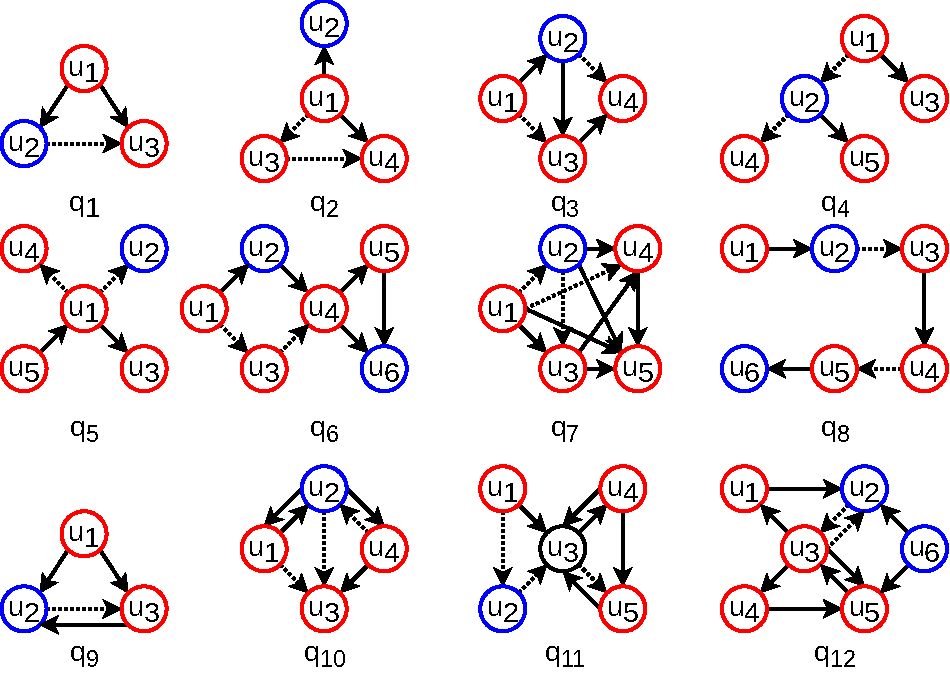
\includegraphics[width=0.5\textwidth]{img/queries.pdf}
  \caption{The queries.}\label{img:queries}
\end{figure}

\subsection{Preprocessing Cost}
We first study the preprocessing cost of SeqStar's vertex-centric storage engine.
The preprocessing incurs a external sort on the original graph data to generate the formatted data graph shown in Figure~\ref{img:data_graph}.
The cost is $\mathcal{O}(n \log n)$ where n is the size of the unsorted graph data.
We use 32-bit integers to store the vertex IDs, and 16-bit integers to store the vertex/edge labels.
As is shown in Figure~\ref{img:exp_preprocessing}, the preprocessing time grows linearly with respect to the size of graph data.
In fact, the preprocessing time of the vertex-centric storage is significantly smaller than the execution time of complex queries.

\begin{figure}[ht]
  \centering
  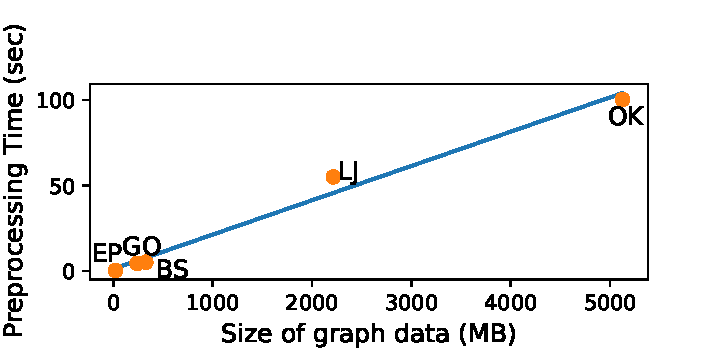
\includegraphics[width=0.4\textwidth]{img/exp_preprocessing.pdf}
  \caption{Preprocessing time of SeqStar.}\label{img:exp_preprocessing}
\end{figure}
\subsection{Comparative Performance}
We compare the overall performance of SeqStar against Graphflow~\cite{DBLP:journals/pvldb/MhedhbiS19} and Neo4j.

Graphflow is the state-of-the-art in-memory subgraph querying system,
and it is the fastest baseline we are aware of.
Graphflow is a JVM based system, and we set the maximum size of the JVM heap to 60GB to let it make full use of main memory.
However Graphflow does not support queries with multi-edges, i.e., $q_9$ --- $q_{12}$,
and it will report fake results for these queries\footnote{Graphflow will report matchings even the data does not contain multi-edges.}.
Therefore we use only $q_1$ --- $q_8$ to compare with Graphflow.
\begin{figure*}[ht]
  \centering
  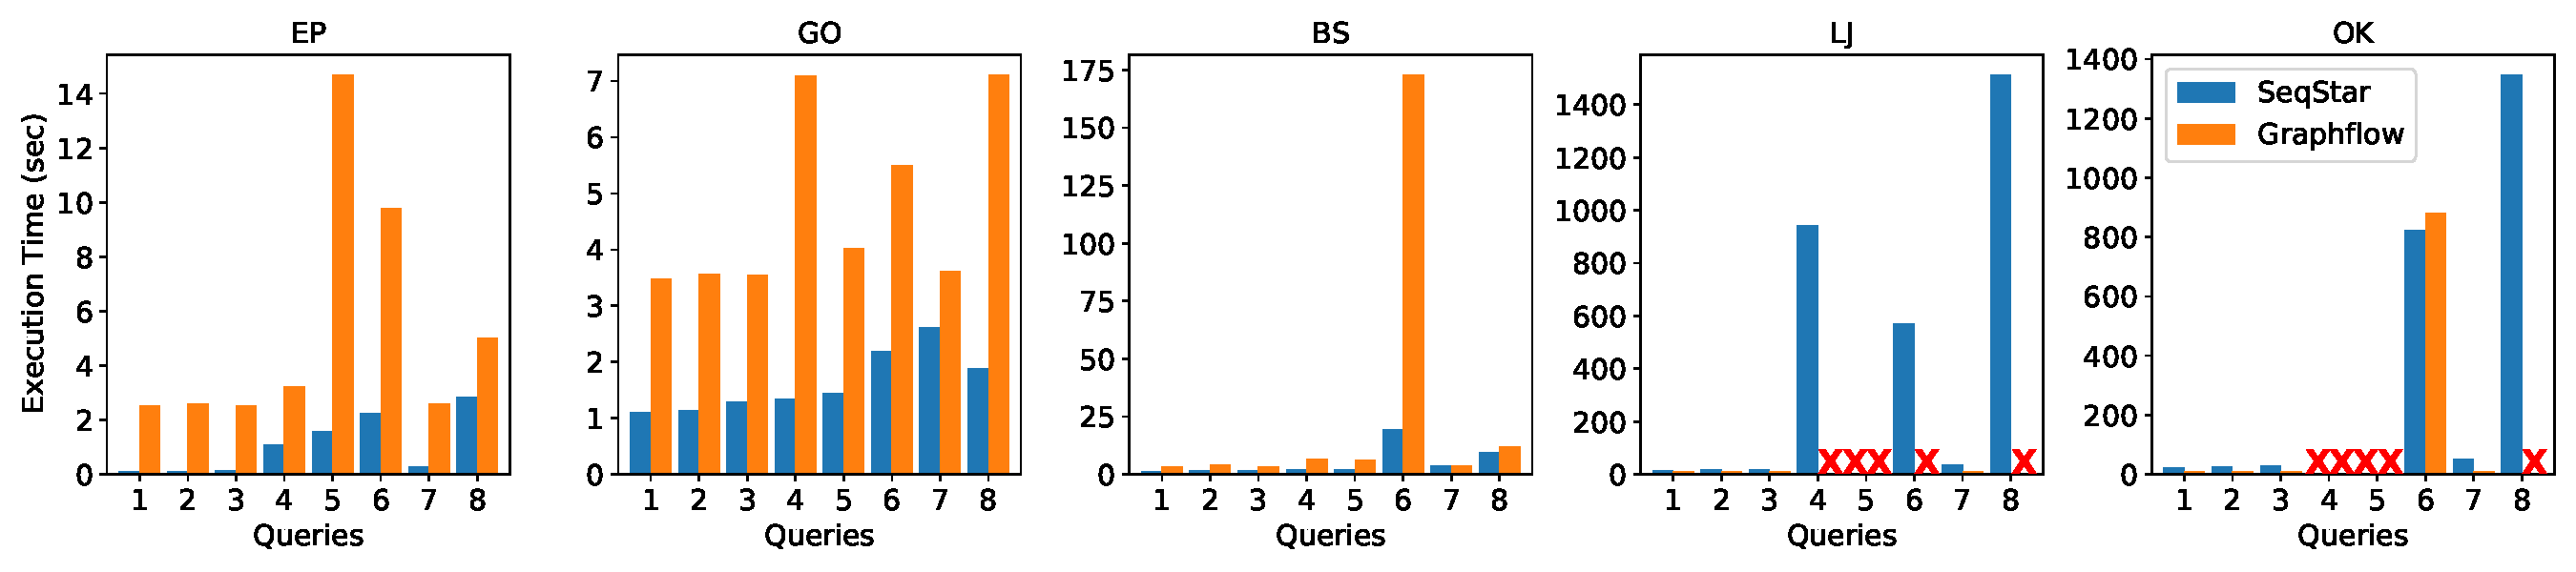
\includegraphics[width=\textwidth]{img/exp_compare.pdf}
  \caption{Execution time.}\label{img:exp_compare}
\end{figure*}

\subsection{Compression Ratio}
\subsection{Performance of Star Decompression}
\subsection{Parallelism of Pipeline Join}

\section{Related Work}
Despite the fact that general property graph matching problem is seldom discussed in previous works,
simple graph matching has been widely studied.
We survey these relevant work in this section.
\subsection*{In-memory Methods}
Most of the early work assumes that the data graph and indices are fit in the main memory of a single machine.
Sparked by Ullmann's backtracking algorithm~\cite{DBLP:journals/jacm/Ullmann76},
many subgraph matching algorithms have been proposed using different searching order, filter rules, and neighborhood indices~\cite{DBLP:journals/pami/CordellaFSV04,DBLP:journals/pvldb/ShangZLY08,DBLP:conf/sigmod/HeS08,DBLP:conf/sigmod/HanLL13,DBLP:journals/pvldb/LeeHKL12}.
These algorithms usually use a DFS-style tree-based graph exploration to search the matchings without materializing intermediate results.
However, these single machine in-memory algorithms are no longer suitable for nowadays billion-node graphs.

To address the scalability problem of single machine in-memory algorithms,
many distributed subgraph matching algorithms have been proposed~\cite{DBLP:journals/pvldb/SunWWSL12,DBLP:conf/sigmod/ShaoCCMYX14,DBLP:journals/pvldb/LaiQLC15,DBLP:journals/pvldb/LaiQLZC16,DBLP:conf/cloud/SerafiniMS17}.
Because the vertices of the data graph are scattered among machines,
these algorithms usually match smaller patterns and get the final result by join operation.
For example, Sun et al.~\cite{DBLP:journals/pvldb/SunWWSL12} introduce a star-like basic matching unit called STwig,
and implement their subgraph matching algorithm on top of the Trinity~\cite{shao2012the} memory cloud.
Lai et al.~\cite{DBLP:journals/pvldb/LaiQLC15} propose TwinTwig join using MapReduce,
where a TwinTwig is either a single edge or two incident edges of a vertex.
The SEED~\cite{DBLP:journals/pvldb/LaiQLZC16} algorithm use both star and clique as the join units,
and use clique compression technique to further improve the performance.
However, these distributed algorithms still suffer from severe memory crisis,
because the size of partial results grow exponentially with respect to the size of the date graph.
Moreover, they must be transferred to other machines before join,
which is the most expensive operation in a parallel system such as MapReduce.

Besides, the optimization of a subgraph matching algorithm relies heavily on the underlying graph model:

Unlabeled undirected simple graph is perhaps the simplest graph model,
which can be viewed as a special case of property graph with all the vertices and edges have the same label and have no multi-edges.
Some authors distinguish this kind of graphs from others and designate the matching problem of this kind of graph as \emph{subgraph listing}~\cite{DBLP:conf/sigmod/ShaoCCMYX14,DBLP:journals/jacm/Ullmann76,DBLP:conf/sigmod/ShaoCCMYX14,DBLP:journals/pvldb/LaiQLC15,DBLP:conf/sigmod/KimLBHLKJ16,DBLP:journals/pvldb/LaiQLZC16,DBLP:journals/pvldb/QiaoZC17}.
CBF~\cite{DBLP:journals/pvldb/QiaoZC17} is the state-of-the-art subgraph listing algorithm,
which decompose the pattern graph into a several basic structures called \emph{crystals},
and match these basic units with partial results compressed by the VCBC algorithm.
However, it is unable to support general property graph because CBF relies on clique listing to match crystals,
which implies the equivalence of vertices in a clique (complete graph) and is not the case of property graph model because of labels and direction of edges.

Another widely studied graph model is vertex-labeled undirected simple graph~\cite{DBLP:journals/pvldb/ShangZLY08,DBLP:journals/pvldb/SunWWSL12,DBLP:conf/sigmod/HanLL13,DBLP:conf/cloud/SerafiniMS17,DBLP:conf/sigmod/DiasTGM019}.
Turbo\textsubscript{ISO}~\cite{DBLP:conf/sigmod/HanLL13}, for example, is turbocharged by the concept of \emph{neighborhood equivalence class} (NEC).
It outperforms other competitors by safely avoid the permutation of all possible vertices in the same NEC\@.
A NEC is a set of vertices in the pattern graph, where every vertex has the same label and the same set of neighbors.
However, things become more complex and make it not suitable for the property graph model.
Because one has to check the labels of vertices, labels of edges, directions of edges in order to test the isomorphism of a property graph, and the real-world multigraphs make life even harder.
\subsection*{Out-of-core Methods}
Many out-of-core triangle enumeration algorithms have been proposed~\cite{DBLP:conf/kdd/ChuC11,DBLP:conf/osdi/KyrolaBG12,DBLP:conf/sigmod/HuTC13,DBLP:conf/sigmod/KimHLPY14}.
However, all these algorithms only deal with triangulation, a special case of the graph matching problem.
Recently, \textsc{DualSim}~\cite{DBLP:conf/sigmod/KimLBHLKJ16} take a further step and is able to match general unlabeled undirected graphs.
To avoid the materialization of intermediate results,
it fixes the data vertices by fixing a set of disk pages and then find all matchings in these pages.
Apparently, every page of the data graph must be swapped in/out many times in order to get the final result,
which lead to severe I/O cost.
In contrast, our approach will load the pages sequentially at most once,
and we can also use the compressed partial results to boost afterward queries.

\section{Conclusion}\label{sec:conclusion}
\textcolor{red}{This paper proposes SeqStar, an out-of-core property graph matching system.}
%This paper proposes SeqStar, which is the first out-of-core property graph matching system.
SeqStar uses the vertex-centric storage engine to store the information related to one vertex together.
This storage engine avoids the random disk access problemand provides the convenient iterators for programs to visit the required vertices.
Small indexes are designed to further minimize the number of IO operations.
For the graph matching engine,
SeqStar uses a novel star decomposition algorithm that preserves as much filtering information as possible in decomposed stars from the pattern graph.
Predicate pushdown is applied to further reduce unnecessary matchings.
In order to reduce the memory usage, SeqStar compresses the intermediate results by postponing Cartesian product and combining equivalent vertices.
And SeqStar performs parallel pipeline join on the compressed data to avoid unnecessary intermediate results.
Experimental results demonstrate that SeqStar outperforms existing work and is able to run more complex property graph queries with less memory consumption.


Currently, SeqStar lacks the support for dynamic graphs.
This limitation gives us directions for future work,
and we are now working on implementing the dynamic vertex-centric storage model to support dynamic graphs.
% 这里扯了一下 future work,看其他的 VLDB 都要在这说,甚至有的这整章就是 future work


%\clearpage

\bibliographystyle{ACM-Reference-Format}
\bibliography{refs}

\end{document}
\endinput
